%Forskning visar på att UX ska ses som ett paradigm inom forskningsvärlden där man ska se det i ett bredare kontext \cite{Bargas-AvilaOldExperience}. UX rollen är bred och beroende på företag samt projekt där man som UX:are tar på sig olika roller, därför tycks många forskare angripa hur essentiellt det är att ha rätt team. \cite{UngerDESIGNLiability} För att få ett bra samarbete inom teamet krävs det rätt kompetens, indelning mellan rollerna, öppen kommunikation inom teamet och följsamhet från utvärderingsmetoder där man validerar och lär sig av de bristfälligheter som tas fram från testning. 

\section{Teori}
I detta avsnitt presenteras teori för forskningsområdet UX och andra väsentliga teorier för denna rapport. Det som kommer att presenteras Människocentrerad Design, Användarcentrerad design, Människa- datorinteraktion, User Expreience, Testning och utvärdering och slutligen  Kategorisering. Denna teori är grundläggande för att kunna förstå begrepp som används i studien.

\subsection{Människocentrerad Design}
Människocentrerad design är en process som har sina rötter i fält som datorvetenskap, ergonomi och artificiell intelligens \cite{Giacomin2014WhatDesign}. Det är således inte en designstil utan är en process som grundar sig på information om människor som ska använda eller nyttja en produkt\cite{Millot2014Human-CenteredDesign}. 
\newline

Människocentrerad design utgår från fysiska och psykiska behov hos mänskliga användare\cite{Millot2014Human-CenteredDesign}. Med det menas att användaren interagerar med en produkt eller tjänst på ett så mänskligt sätt som möjligt, så att användandet inte blir ett hinder. Produkten eller tjänsten tillgodoser behov och förmågor hos användaren och designen anpassas därefter\cite{Millot2014Human-CenteredDesign}.  ISO 9241-210 \textit{Ergonomics of human-centred system interaction} beskriver människocentrerad design som\cite{ISOSystems}: 
\newline

\begin{quotation}
\em{Approach to systems design and development that aims to make interactive systems more usable by focusing on the use of the system and applying human factors/ergonomics and usability knowledge and techniques}
\newline
\end{quotation}

Datorsystem är en typ av interaktivt system och karakteriseras av ett signifikant antal interaktioner mellan människa och dator \cite{InteractiveDictionary}. Interaktiva system är något som behöver vara användbart, lättförståeligt och som får användaren till fortsatt användning\cite{May2012ApplyingApp}. Interaktiva system är således något som måste utgå från människocentrerad design\cite{Human-CenteredStudio}. 

\subsection{Användarcentrerad design}

Människocentrerad design blandas ofta ihop med termen användarcentrerad design\cite{Abras2004User-CenteredDesign}. Användarcentrerad design fokuserar på en djupare analys av målgruppen, specifika egenskaper och specifika egenskaper hos målgruppen . Detta är en fas där målgruppen spelar stor roll i designprocessen. De aspekter som bör tas till hänsyn vid utformning av designen är; specifik målgrupp, kön, ålder, social status, utbildningsnivå och professionell bakgrund\cite{Human-CenteredStudiob}.Utifrån de aspekterna bör en djupgående analys göras och specifika preferenser tas till hänsyn. Dessa preferenser kan vara exempelvis; känslomässiga och fysiska uppfattningsdrag samt nivåer av teknikmedvetenhet och många andra faktorer\cite{Human-CenteredStudiob}. 
\newline

\subsection{Människa- datorinteraktion}

Människa- datorinteraktion (MDI) är ett forskningsområde som studerar interaktionen mellan människa och dator\cite{Blanton2009Human-ComputerInteraction}. Forskningsområdet etablerades på tidigt 60-tal men det var inte förrän på 80-talet som termen Människa- datorinteraktion fick sin spridning\cite{Myers1998ATechnology}. Idag ses MDI och dess begrepp som en nödvändighet för att utforma interaktiva system\cite{TheCambridge}. 
\newline

Forskningsområdet MDI har haft många namn så som; mänskliga faktorer, ergonomi, kognitiv ergonomi, människa-maskin interaktion etc \cite{Smith-Atakan2006Human-computerInteraction}. En bättre etikett på forskningsområdet beskrivs av Pinker \cite{Langendoen1999HowWorks} Han föredrar att kalla forskningsområdet "naturlig beräkning". Han menar att "naturlig beräkning" refererar till beteendes som är naturliga för människan, med eller utan extern hjälp, för informationsprocessen samt hantera naturliga symboler.  
 
\subsubsection{Användbarhet}
Ett centralt begrepp inom människa- datorinteraktion är användbarhet. Begreppet är en mätning på hur väl användaren kan interagera med eller använda ett system \cite{Blanton2009Human-ComputerInteraction}.
För att uppnå en god användbarhet krävs det att man arbetar med människocentrerad design\cite{BenyonDesigningDesign}. Ett sätt att se på användbarhet är uppnå en balans mellan de fyra principerna i MAST (engelska PACT)\cite{BenyonDesigningDesign}: 

\begin{itemize}
\item Människor
\item Aktiviteter människor vill göra
\item Sammanhang där samspelet äger rum
\item Teknologin (hård- och mjukvara)
\end{itemize}

Dessa fyra principer är faktorer som spelar stor roll i människocentrerade interaktiva system där användbarhet är ett faktum.
\newline

Norman  definierar begreppet användbarhet i interaktiva system efter fem kvalitativa komponenter\cite{UsabilityUsability}: 
\begin{itemize}
\item \textbf{Lärande ändamål}: hur enkelt är det för användaren att utföra enkla uppgifter? 
\item\textbf{Effektivitet:} hur snabbt kan uppgiften utföras när användaren lärt sig designen? 
\item \textbf{Minnesvärdighet:} när användaren återvänder till designen efter en period, hur snabbt kan användaren återkoppla till uppgiften? 
\item\textbf{Misstag:} hur många misstag gör användaren och hur kan de ta igen sig efter misstaget?
\item\textbf{Tillfredsställelse:} hur behaglig känns designen att använda? 
\end{itemize}

Han menar att dessa komponenter är viktiga för användbarheten av olika system för att användaren inte ska lämna eller överge systemet. 
 

\subsection{User Experience}
User Experience, direkt översatt till svenska är \textit{användarupplevelse} vilket är precis som ordet beskriver, den personligt upplevda känslan och tanken vid användning av en produkt eller tjänst \cite{Bargas-AvilaOldExperience}. Det innebär att UX är en viktig del av den värdeskapande processen av en produkt eller tjänst och har som mål att ge meningsfulla och bra upplevelser för användaren\cite{FlaveDesignprinciperMarknadsplats}. På ett generellt plan så handlar UX området om den helhetsbild som fås av en tjänst eller produkt samt huruvida människor kommer att använda den och vad som attraherar användaren till att nyttja en produkt eller tjänst \cite{Bargas-AvilaOldExperience}. Sheng och Teo \cite{Sheng2012ProductExperience} menar på att resultatet av User Experience, som metod, bygger på en bedömning mellan skillnader. Dessa skillnader är vad en kund förväntar sig och den stimuli som resulterar från en interaktion mellan företaget och dess produkt eller service som speglar kontrapunkterna mellan båda parter. 
\newline

Det finns många olika definitioner på vad UX är, men en person som har haft en betydande roll för forskningsområdet är Norman som beskriver UX som följande \cite{NormanTheUX}:
\newline
\begin{quote}
\em 
All aspects of the end-user’s interaction with the company, its services, and its products. The first requirement for an exemplary user experience is to meet the exact needs of the customer, without fuss or bother. Next comes simplicity and elegance that produce products that are a joy to own, a joy to use. True user experience goes far beyond giving customers what they say they want, or providing checklist features. In order to achieve high-quality user experience in a company’s offerings there must be a seamless merging of the services of multiple disciplines, including engineering, marketing, graphical and industrial design, and interface design. 
\newline
\end{quote} 

Med andra ord, User Experience omfattar alla aspekter av slutanvändarens interaktion med företaget, dess tjänster och produkter \cite{NormanTheUX}. 
\newline

Som tidigare nämnt har UX många definitioner och en anledning till det är att forskare anser att det är ett komplext forskningsområde\cite{20Mastery}. På senare år har det påståtts att UX är där affärsbehov och användaren möts, och genom att ställa centrala frågor så som \textbf{vad}, \textbf{varför} och \textbf{när} då utformning av en produkt görs och dessutom fokusera på att arbeta användarcentralt så underlättar man designprocessen\cite{20Mastery}. 
\newline

Interaktionsdesign är ett ungt fält som fortfarande försöker hitta sin plats bland andra systerfält så som informationsarkitektur (IA), industriell
design (ID), visuell (eller grafisk) design, användarupplevelse (UX) design och mänskliga faktorer\cite{SafferCreatingDevices}. Figur 1 klargör
förhållandet mellan dem, enligt Saffers så faller de flesta fält faller under User Experience, \enquote{disciplinen att titta på alla aspekter} \cite{SafferCreatingDevices}.

\begin{figure}[H]
  \centering
  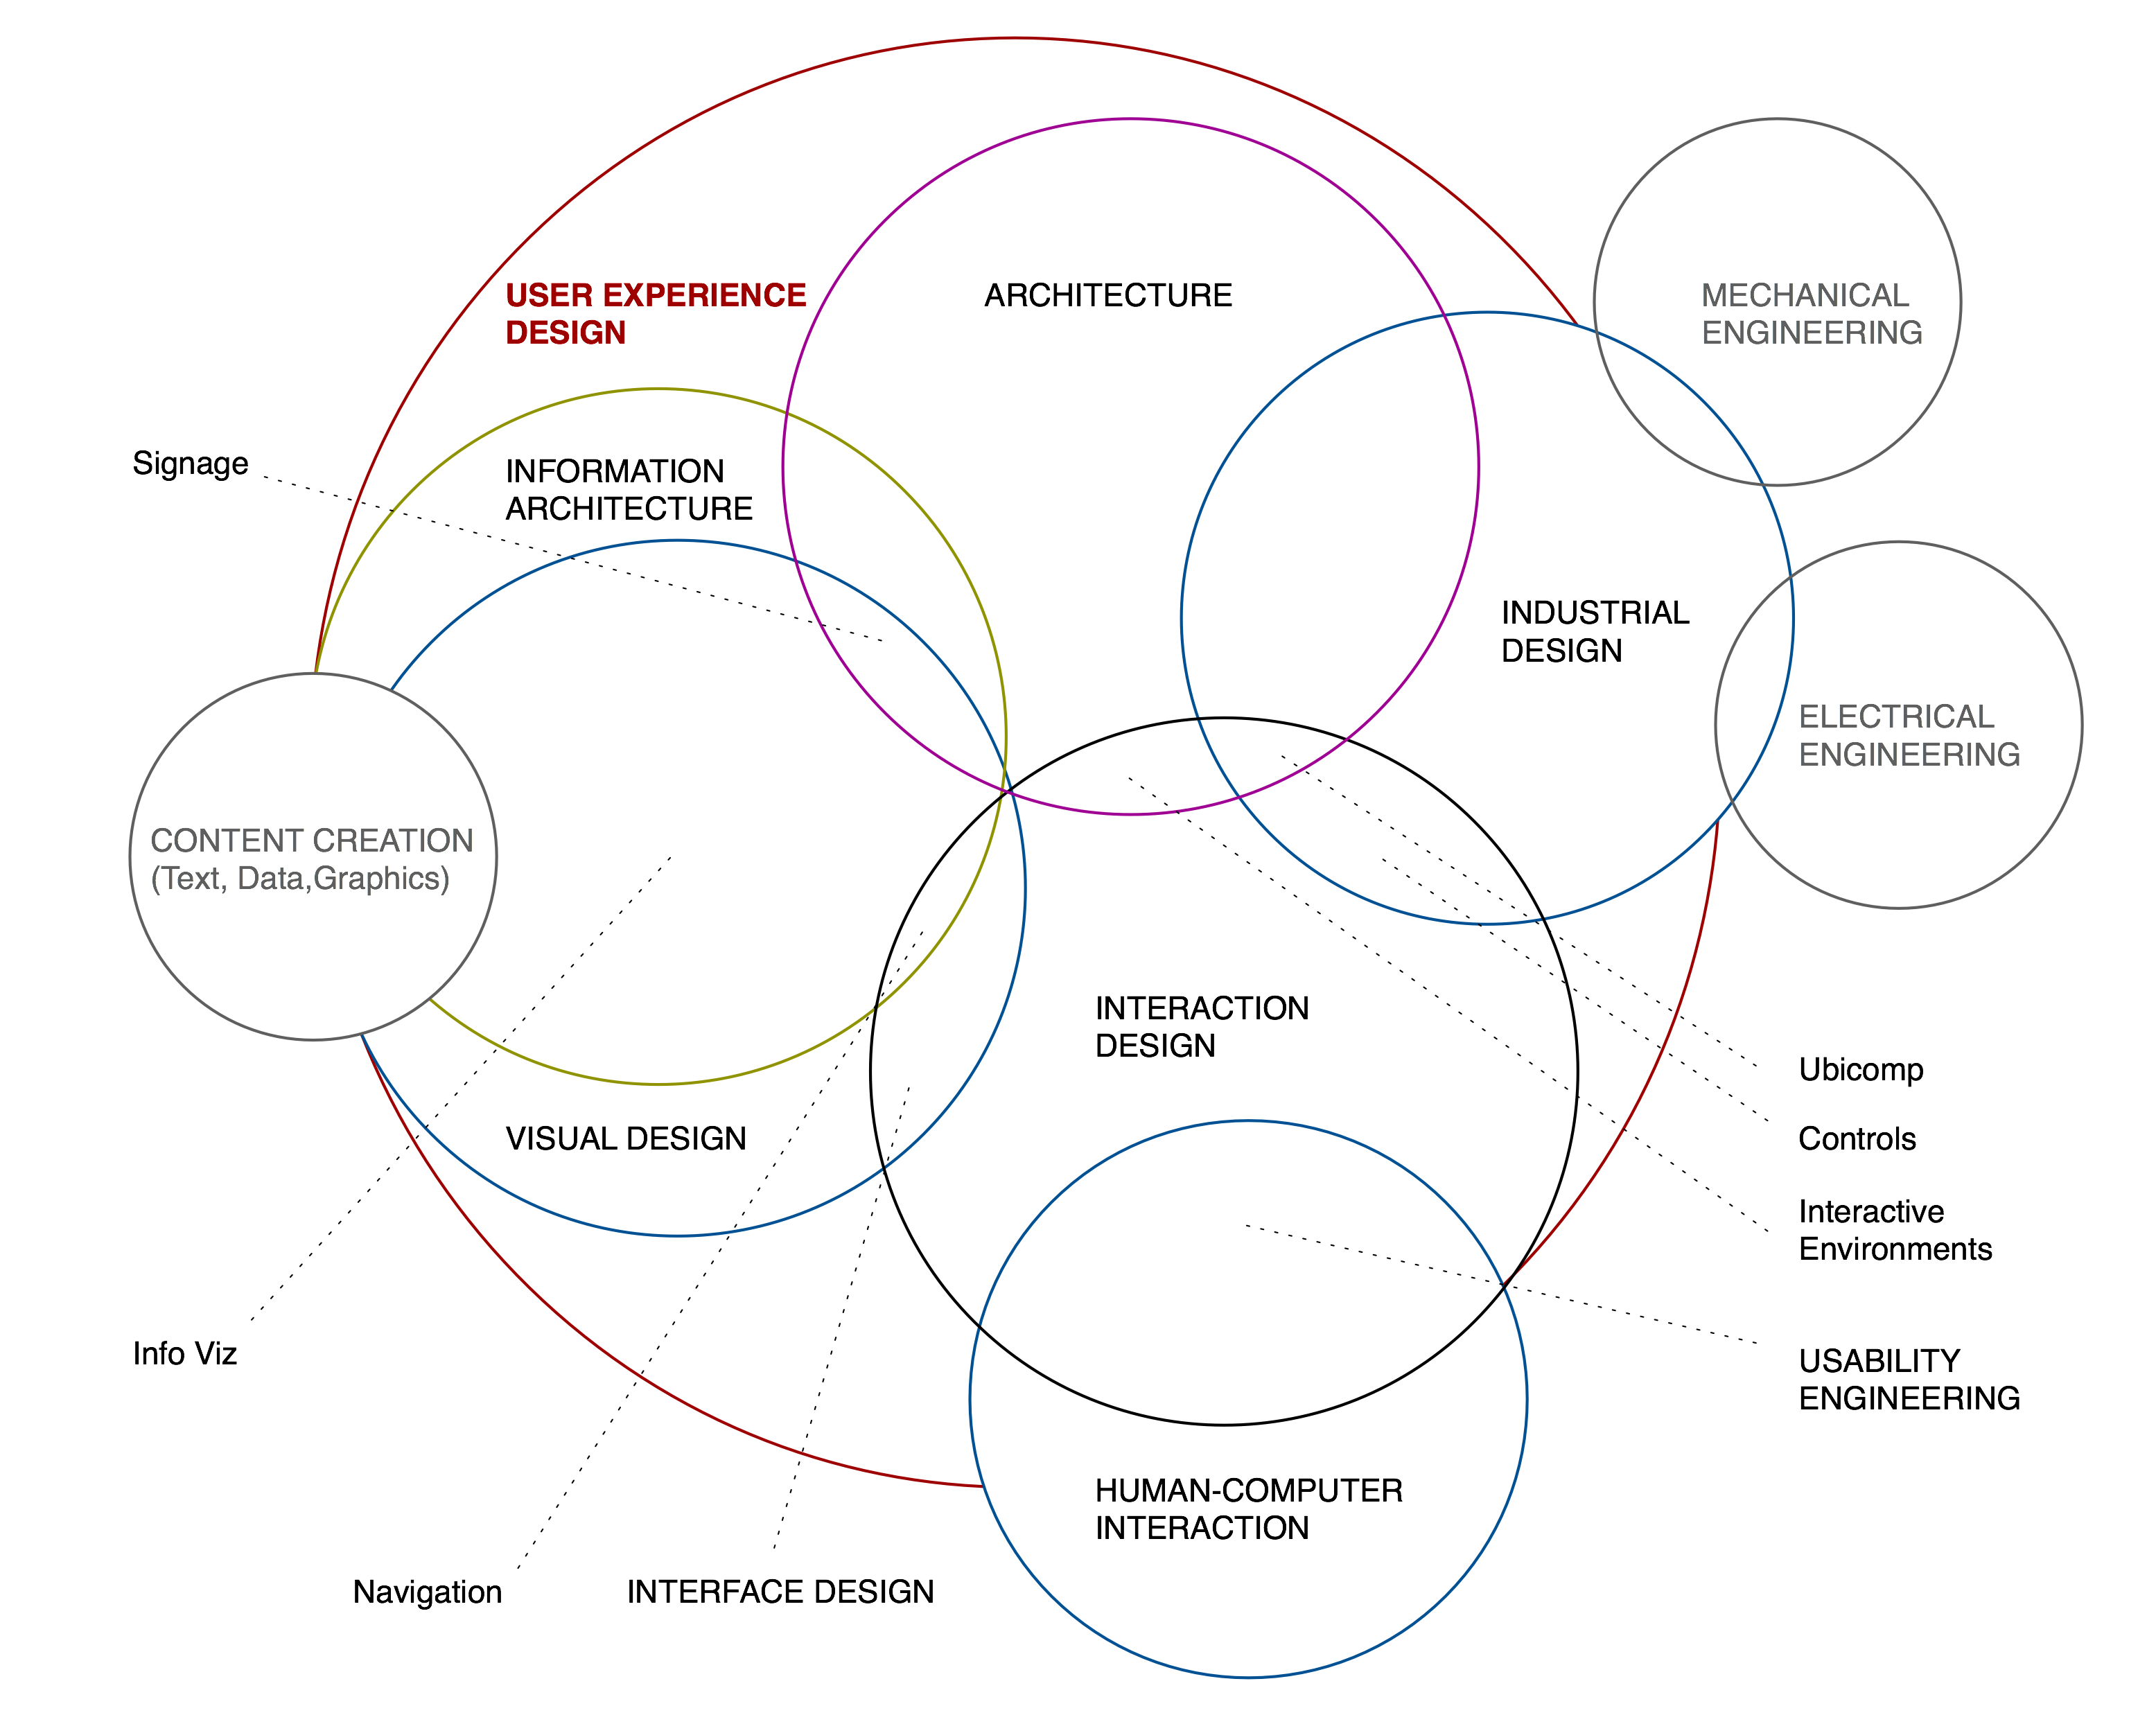
\includegraphics[scale=0.45]{ux.jpg}
  \caption{Saffers definition på UX\cite{SafferCreatingDevices}}
\end{figure} 

Norman säger att design kräver kunskap från flera områden vilket gör UX subjektivt och dess utvärderingsmetoder subjektiva \cite{NormanquotPeople}. Dillon menar att den upplevda användbarheten och dess tillfredsställande estetik är två kriterier som behövs ta hänsyn till för att förstå User Experience, medan andra forskare menar på att fokus bör vara på att arbeta med personen i sig \cite{Lee2010UnderstandingUse}. 

UX-området tar till hänsyn att värdesätta användarens upplevelse av en produkt eller tjänst vilket kan innebära att användaren gör ett ställningstagande runt dess estetik\cite{TuchIsHCI}. Det finns en växelverkan mellan hedonistiska faktorer och helhetsupplevelser av system \cite{TuchIsHCI}.
\newline


\subsubsection{Vår syn på User Experience}
Då User Experience har många definitioner har vi valt att tolka området på vårt sätt utifrån den fakta som samlats in. Enligt Bargas \cite{Bargas-AvilaOldExperience} är User Experience den personligt upplevda känslan kring en produkt eller tjänst, vilket också är sättet vi har tolkat UX på. Då det är viktigt att användaren kan interagera med en produkt eller tjänst på ett så enkelt sätt som möjligt så är en av grundprinciperna att sätta användaren i fokus. Detta är något vi samtycker med då många företag tenderar att implementera tjänster utefter deras behov istället för användaren \cite{PlaneradBokhandel}. Detta leder till funktionaliteter som inte uppnår användaren behov och tjänsten/produkten riskerar att inte bli nyttjad.
\newline

Det är viktigt med en tydlig distinktion mellan användbarhet och User Experience. De har mycket gemensamt, men UX tar till hänsyn att värdesätta användarens upplevelse av produkten och dess vilja att nyttja den. Detta kan innebära att användaren tar ett ställningstagande runt dess estetiska tilltalet, det vill säga om den är väldesignad och om användaren upplever att den är hedonistiskt tillfredsställande. Det finns samband där en god användbarhet har influerad testpersonens åsikt om den upplevda estetiken\cite{Gualtieri2009BestDesign}. Forskning visar på att en växelverkan mellan hedonistiska faktorer och helhetsupplevelser av system existerar\cite{TuchIsHCI}. Det är viktigt att icke-funktionella inslag av en produkt tas till hänsyn, där man gör en distinktion mellan användbarhet och UX. 
\newline

\subsection{Prototyper}
Att få en design perfekt vid första försöket är omöjligt vilket är allmänt känt för yrkesverksamma inom UX. Därför används prototyper i ett tidigt skede då man vill utvärdera design och funktionalitet \cite{Yamakami2014ExploratoryDesign}. För att få en god användarupplevelse behövs det utformas en testmodell. I kontext till denna studien är testmodellen en prototyp. I dess tidigaste skede, innan utveckling av kod görs, börjas det med skisser eller low-fidelityprototyper \cite{Gualtieri2009BestDesign}. Gualtieri\cite{Gualtieri2009BestDesign} förespråkar att utforma (designa) ett koncept i ett tidigt skede och använda sina slutanvändare för att utveckla designen vidare (läs mer om detta i sektion 2.6 Användartestning och utvärdering). Vad en prototyp är kan skilja sig oerhört, från att vara en välutvecklad interaktiv prototyp till en skiss på ett papper\cite{HoudeWhatPrototype}. Grundreceptet är att det går att testa och validera på slutanvändaren för att förstå hur det ska gås vidare i design och utvecklingsprocess\cite{HoudeWhatPrototype}.
\newline

Enligt Houde och Hill \cite{HoudeWhatPrototype} är en prototyp något som är till för att utforska och visa en design. De menar att det är en vedertagen metod att bygga en prototyp för att representera något i de olika stadierna av designen, och för att utforska möjligheter. Emellertid är interaktiva system komplexa där det kan vara svårt att skapa prototyper av en hel design \cite{HoudeWhatPrototype}.
\newline

Modellen i figur 2 är en bild som ska representera de viktigaste aspekterna i en design av en interaktiv prototyp. Bilden representerar Houde och Hill:s syn på vad en prototyp är och de menar på att de tre aspekterna som man bör ha i åtanke är\cite{HoudeWhatPrototype}:
\begin{itemize}
\item Rollen
\item Hur den ser ut och känns
\item Implementationen
\end{itemize}
Med \enquote{rollen} syftar de till frågor om funktionaliteten som har med användaren att göra. 
\enquote{Hur den ser ut och känn} har att göra med den konkreta upplevelsen om användarens estetiska intryck och hur användaren anser att den känns. Med \enquote{implementation} syftar Houde och Hill till frågor angående tekniken och de som kallar för UI (User Interface). Triangeln är gjord för att enkelt kunna visa vilka aspekter som är viktiga samt att ingen del är mer essentiell än den andra. Målet med modellen är att vid ett designproblem (oberoende av storlek eller dess omfång) ska triangeln behandlas som ett hjälpmedel för att separera diverse problem in i dessa tre klasser. Detta för att förstå de frågor varje klass sekventiellt ställs inför.

\begin{figure}[H]
  \centering
  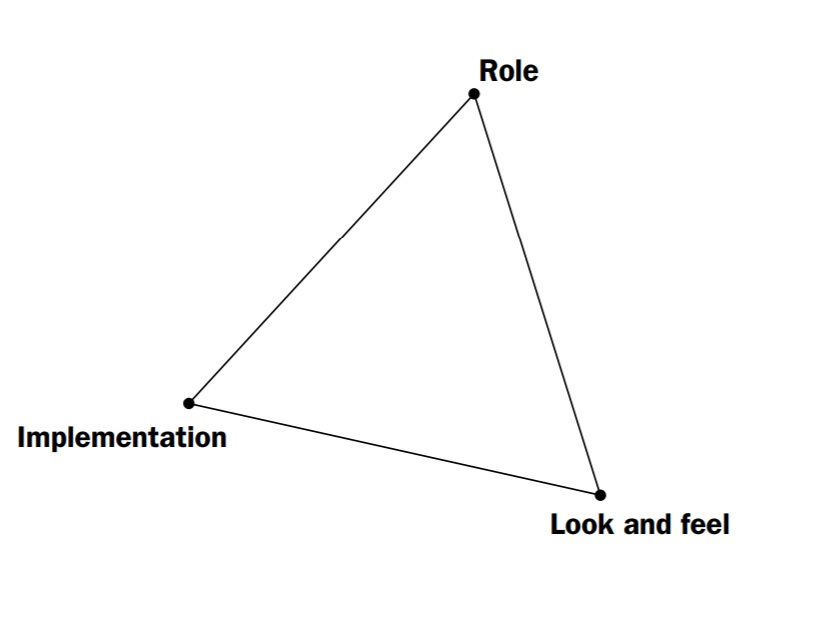
\includegraphics[scale=0.9]{resources/Prototyp.jpg}
  \centering
  \captionsetup{justification=centering, margin=2cm}
  \caption{Figur från \textit{What do Prototypes Prototype?} av Stephanie Houde och Charles Hill
 \cite{HoudeWhatPrototype} }
\end{figure}

Genom att explicit fokusera på vissa designfrågor kan man förstå vilken typ av prototyp som ska implementeras, hur den ska testas och vilken modell som hjälper att visualisera det fokus som ska vara efter utformning av syftet med applikationen\cite{HoudeWhatPrototype}. Således är de frågor man ska ställa sig, enligt Houde och Hill\cite{HoudeWhatPrototype}: 
\begin{itemize}
\item Vilken roll kommer det att spela i användarens liv?
\item Hur ska det se ut och känna? 
\item Hur bör det genomföras?
\end{itemize}

 Figur 2 och dess attribut är ett verktyg som kan användas för att prototypen ska uppfylla de syfte man vill att den ska göra -där olika prototyper har olika indelningar i de tre klasserna och svar på de frågorna ger en specifik fördel vid utformandet av den \cite{HoudeWhatPrototype}.


\subsection{Användartestning och utvärdering}
En mängd olika metoder har utvecklats för att stödja människocentrerad och användarcentrerad design\cite{Abras2004User-CenteredDesign}. Dessa metoder är bland annat användartester, heuristisk utvärdering, diskussionsutvärdering och deltagande design. 
\newline

Användartestning är en central del inom UX som betyder att man sätter slutanvändaren i centrum. Detta för att kunna undersöka om prototypen eller produkten når upp till kriterierna för god användbarhet och användarupplevelse för slutanvändaren\cite{Gualtieri2009BestDesign}.  En riktlinje som Gualiteri går in på är att man inte ska lita på någon, utan testa allt, där testresultat kan ge konkreta värden och väsentlig riktning av ett projekt\cite{Gualtieri2009BestDesign}.  
\newline
 
När en digital plattform formas behövs det utföras användartestning för att nå förväntningarna som en användare har på produkten. Gualtieri \cite{Gualtieri2009BestDesign} menar att det behövs göras vid ett tidigt skede när utformning av en produkt eller tjänst görs, så att man kan förstå användaren. Han menar också att användartestning ger resultat som kan ge riktlinjer som är essentiell vid utformningen av applikationen. Han nämner också att man lätt förväxlar kunden och slutanvändaren, då dessa nödvändigtvis inte delar samma behov eller mål. För att kunna utföra användartester krävs det att det finns något att testa på så som en modell, prototyp eller del av en applikation\cite{Gualtieri2009BestDesign}. Vredenbrug \cite{Vredenburg2002APractice} gjorde en fallstudie där han kom fram till att en iterativ design är en grundpelare för att få en användarcentrerad utveckling. 
\newline

Ett problem, som är viktigt att ha i åtanke vid utformning av ett användartest, är att den del/modell eller prototyp som testas på användaren bör vara väl fungerande där funktionaliteten inte ska vara begränsad till den utsträckning att det påverkar det estetiska tilltalet{\cite{Gualtieri2009BestDesign}. Det är viktigt att icke-funktionella inslag av en produkt tas till hänsyn vid användartester, där man gör en distinktion mellan användbarhet och användarupplevelse. Det är därmed viktigt att vara tydlig med syftet av användartestningen, så att man inte har fokus på funktionalitet utan fokus är på helhetsbilden av användarupplevelsen.
\newline

Enligt Benyon \cite{Benyon2013Designing3/E} är det viktigt att förstå att en undersökning i form av intervju eller enkät inte är tillräcklig, utan detta ska ske i kombination med observation för ett korrekt resultat. Testpersonen ska representera slutanvändaren, vilket betyder att hen nödvändigtvis behöver vara just den exakta slutanvändaren utan behöver tänka som slutanvändaren \cite{Benyon2013Designing3/E}.
\newline

\subsection{Kategorisering}
\label{kategorisering}
Människocentrerad design och användarcentrerad design är två ramverk som kan användas i varje vid utformning av produkt eller tjänst. Genom att använda ett UX-ramverk kan man på ett strukturerat sätt ta in alla dess olika attribut. Då UX definieras på många olika sätt så kan det vara en trygghet att luta sig mot ett studerat och testat ramverk. 
\newline

Konstruktionen av frågeformuläret samt frågorna till fokusgrupperna baseras Laugwitz, Held, och Schrepp's artikel "Construction and Evaluation of a User Experience
Questionnaire" \cite{Laugwitz2008ConstructionQuestionnaire}. Dem i sin tur utgick efter ett teoretiskt ramverk inom User Experience \cite{HassenzahlUserQuality}. Ramverket är framtaget av Hassenzahl och syftar till att gruppera två olika kvalitetsaspekter: ergonomisk kvalitet (EQ) och hedonisk kvalitet (HQ)\cite{HassenzahlUserQuality}. Ramverket särskiljer på upplevd ergonomisk kvalitet och upplevd hedonisk kvalitet. Detta används sedan för att kunna utvärdera hur attraktiv en produkt eller tjänst är, enligt Hassenzahl. 
\newline

Uppkomsten av Hassenzahls ramverk grundar sig på begreppet användbarhet, inom Människa- datorinteraktion, där han menar att användbarhet inte tillgodoser faktorer om huruvida produkten eller tjänsten är rolig att använda \cite{HassenzahlUserQuality}. Han menar också att användbarhet inte tar hänsyn till preferenser vad det gäller användarens tillfredsställelse. Därför föreslogs en ny modell som inkluderade "hedonisk kvalité" \cite{HassenzahlUserQuality} . 
\newline

Ergonomisk- och hedonisk kvalitet är två kategorier som sammanfattar olika kvalitetsaspekter\cite{HassenzahlUserQuality}. Ergonomisk kvalitet innebär att man ser till den målorienterade eller arbetsorienterade aspekterna i designen av en produkt eller tjänst\cite{HassenzahlUserQuality}. En hög ergonomisk kvalitet innebär att användaren kan nå uppgiftsorienterade mål på ett effektivt sätt\cite{HassenzahlUserQuality}. Hedonisk kvalitet syftar till vad användaren tycker om produktens estetik eller attraktivitet\cite{HassenzahlUserQuality}. Här är aspekter som uppgiftsorienterade mål, jämfört med ergonomisk kvalitet, inte viktigt\cite{HassenzahlUserQuality}. 
\newline

Personer antas således uppfatta flera olika aspekter vid en utvärdering av en produkt\cite{HassenzahlUserQuality}. Kontrapunkten mellan ergonomisk och hedonisk kvalitet bör således tas till hänsyn vid en undersökning av en produkt\cite{Laugwitz2008ConstructionQuestionnaire}. Enligt detta antagande bör frågeformuläret innehålla två indelningar enligt Laugwitz, Held, och Schrepp\cite{Laugwitz2008ConstructionQuestionnaire}:
\begin{itemize}
\item den uppfattade attraktiviteten (EQ) och
\item den uppfattade kvaliteten på relevanta aspekter (HQ).
\end{itemize}

Frågeformuläret som utformades av Laugwitz, Held, och Schrepp arbetades fram med hänsyn till UX-ramverket av Hassezahl \cite{Laugwitz2008ConstructionQuestionnaire}. De arbetade iterativt fram olika kategorier som tog hänsyn till EQ och HQ. Kategorierna omfattade de två indelningarna vid undersökning av en produkt: den uppfattade attraktiviteten och den uppfattade kvaliteten på relevanta aspekter. Tillslut kom de fram till fem kategorier\cite{Laugwitz2008ConstructionQuestionnaire}: 
\begin{itemize}
\item Tydlighet
\item Effektivitet
\item Pålitlighet
\item Stimuli
\item Attraktivitet
\end{itemize}

Dessa kategorier har vi använt som grund till vår analys och utvärdering på AL1 prototypen. 

\subsubsection{Anledning till val av att använda kategoriseringen}

Olika applikationer har mer eller mindre krav beroende på syftet med användandet av applikationen\cite{UXUX}. Dessa krav berör också upplevelsen som användaren har. Ett exempel på detta är en applikation som har att göra med transaktioner, betalningsmetoder eller pengar att göra.I en sådan applikation har användaren höga krav på tydlighet så att funktionaliteten flyter på\cite{UXUX}. Användaren behöver i detta fall uppleva att applikationen är pålitlig, där utseendet (attraktiviteten) inte är ett högt krav\cite{UXUX}. Som Hassenzahl menar, när en användare gör en utvärdering av en applikation så vägs olika egenskaper in vid bedömningen. Forskare inom designteknik, exempelvis Karat, Lindgaard och Bassat\cite{Ben-BassatEconomicUsability}\cite{LindgaardWhatSatisfaction} \cite{Karat2003TheField}, indikerar på att designtekniken har en inverkan på preferenser hos användaren. Således behöver man behärska både syftet med applikationen och vad slutanvändaren anser vara viktigast för användarupplevelsen. Om man vill att applikationen ska vara användarcentrerad behöver man förstå vilken aspekt som är viktigast och göra en prioritering \cite{5Foundation}.
\newline

Det är anledningarna till varför vi valt att arbeta med de kategorier som utformats av Laugwitz, Held, och Schrepp  för att undersöka vad användaren tycker om Amazing Leaders prototyp. 





